\documentclass{article}
\usepackage[a4paper, total={6in, 8in}]{geometry}
\linespread{1.5}
\usepackage{float}
\usepackage[utf8]{inputenc} 
\usepackage[portuguese]{babel} 
\usepackage{amsmath,amsfonts,amsthm}
\usepackage{graphicx}
\usepackage{indentfirst}
\usepackage{natbib}
\usepackage{sectsty} 
\usepackage{graphicx}
\usepackage{float}
\usepackage{listings}
\usepackage{hyperref}


\newcommand{\horrule}[1]{\rule{\linewidth}{#1}} 

\title{	
\normalfont \normalsize 
\textsc{Escola de Matemática Aplicada} \\
\textsc{Fundação Getúlio Vargas}\\ [25pt] 
\horrule{0.5pt} \\[0.4cm]
\huge Trabalho 2 - Computação Escalável\\ 
\horrule{2pt} \\[0.5cm] 
}

\author{Fernanda Luísa Silva Gomes \\ Igor Patricio Michels \\ Laura Chaves Miranda \\ Marcos Antônio Alves \\[0.1cm]{ Professor: Thiago Pinheiro de Araújo}}
\date{27 de junho de 2023} 


\begin{document}
\maketitle 
\section*{Modelagem da arquitetura}

\subsection*{Ambiente local}

Salvo comentários considerados pertinentes, nenhum detalhe de implementação será abordado, uma vez que o foco da seção está na arquitetura do programa.

\subsubsection*{Comunicação entre simuladores e transformadores}

Implementamos Publish-Subscribe como mecanismo de comunicação, por meio da biblioteca \textit{celery} e do broker RabbitMQ. Nessa comunicação são enviados dois tipos de mensagens.

O primeiro é referente às informações da rodovia: código, velocidade máxima permitida, velocidade máxima dos carros (para um cálculo de colisão mais realístico), os limites do intervalo de interesse na análise histórica de direção perigosa, além do número máximo de eventos de risco (N) aceitável nesse intervalo em um tempo T (parametrizado dentro do programa). A escolha pela parametrização de T como constante no programa foi dada em virtude da presença de um termo de mesma ideia na análise onde computamos os carros proibidos de circular. Como tal mensagem apresenta apenas parâmetros específicos (e imutáveis) de cada rodovia, essa mensagem é enviada apenas uma vez, ao instanciar a rodovia.

O segundo tipo de mensagem contém informações do carro: placa, posição, pista, rodovia e horário de emissão. Essa mensagem serve como um rastreador GPS dos carros, sendo o dado que é utilizado para a realização das análises, de acordo com os parâmetros recebidos das rodovias e das constantes definida dentro do programa.

Por fim, os consumidores recebem as mensagem e populam um banco MongoDB com os dados recebidos. Nesse sentido, o banco possuí duas coleções, uma com as informações das rodovias e outra com os dados referentes aos carros.

\subsubsection*{Transformadores e Dashboard}

Após inserção dos dados no MongoDB, o \textit{pyspark} realiza a leitura dos dados presentes nas tabelas. Para análises históricas, todos os dados dos carros são lidos e transformados. Já para análises atuais são realizados filtros de modo que consideramos apenas as últimas três posições de cada carro em sua viagem atual pela rodovia em que ele está. Por fim, com auxílio da biblioteca \textit{psycopg2}, os resultados das análises são armazenados no PostgreSQL, finalizando o fluxo de ELTL e simplificando a conexão com o Dashboard.

Também visando a facilidade de implementação do painel, cada tabela do PostgreSQL corresponde a uma tabela presente no painel. Por último, as bibliotecas \textit{psycopg2} e \textit{streamlit} auxiliam, respectivamente, na leitura dos dados e criação do Dashboard com as análises.

Adiantando um pouco uma decisão de projeto, podemos comentar sobre um detalhe voltado a confiabilidade do programa. O fato de considerar apenas a viagem atual, citado no primeiro parágrafo desta seção, é de extrema importância. Considerando que um veículo pode sair de uma rodovia X e voltar a mesma rodovia após algumas iterações, realizar as análises com lag 2 dos dados poderia resultar em uma velocidade e uma aceleração esdrúxulas, a depender de como o veículo saiu e entrou. Exemplo: o veículo estava na rodovia 100 e saiu da mesma no sentido norte-sul, na posição 10000. Após algumas iterações, o mesmo veículo volta a rodovia 10000, no mesmo sentido, mas no início da rodovia (posição 0), logo sua velocidade é igual a -10000, o que é claramente um equívoco.

Por fim, a Figura \ref{fig:arquitetura_ambiente_local} expressa, de modo abrangente, a arquitetura utilizada no ambiente local.

\begin{figure}[H]
    \centering
    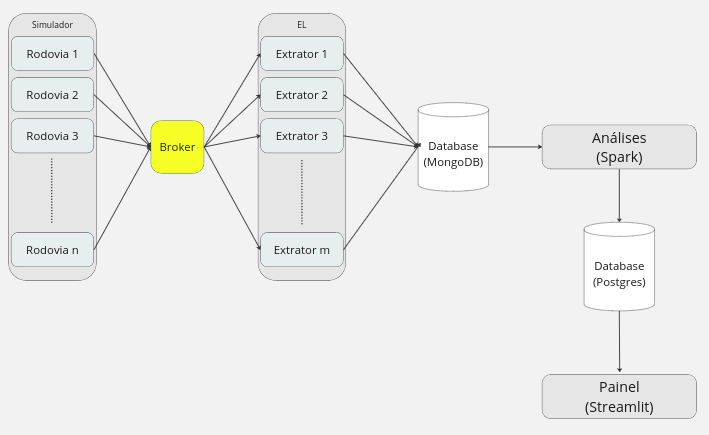
\includegraphics[scale = 0.6]{images/Arquitetura_ambiente_local.png}
    \caption{Arquitetura desenvolvida para execução local}
    \label{fig:arquitetura_ambiente_local}
\end{figure}

\subsection*{Ambiente de nuvem}

Para a implementação do sistema de comunicação na nuvem, utilizaríamos o ECS. Seria criado, por meio do docker, um contêiner baseado na implementação local e adaptado para o ambiente da AWS. Visto que usamos o RabbitMQ como broker, teríamos o AmazonMQ como serviço de gerenciamento de mensagens na AWS para criar uma instância com o RabbitMQ.

O banco de dados MongoDB seria substituído pelo DynamoDB, por também ser um banco não colunar e ajudar na escalabilidade. O pipeline de processamento em Spark seria executado por meio do Amazon Glue. Após transformação, os dados seriam carregados em um banco PostgreSQL através do S3. Por fim, seria necessário adaptar o painel localmente executado com \textit{streamlit} para o AWS Athena.

Iniciamos com uma tentativa de implementação na AWS, com a criação de um dockerfile e de alguns bancos na AWS. Foram criadas duas tabelas no DynamoDB, dentro da AWS e um banco PostgreSQL, mas não foi possível acessar ao AmazonMQ, conforme pode ser observado na Figura \ref{amazonmq}. Nas tentativas realizadas, o ambiente ficava apenas com o status de carregando, com o círculo no canto superior esquerdo da tela.
\begin{figure}[H]
    \centering
    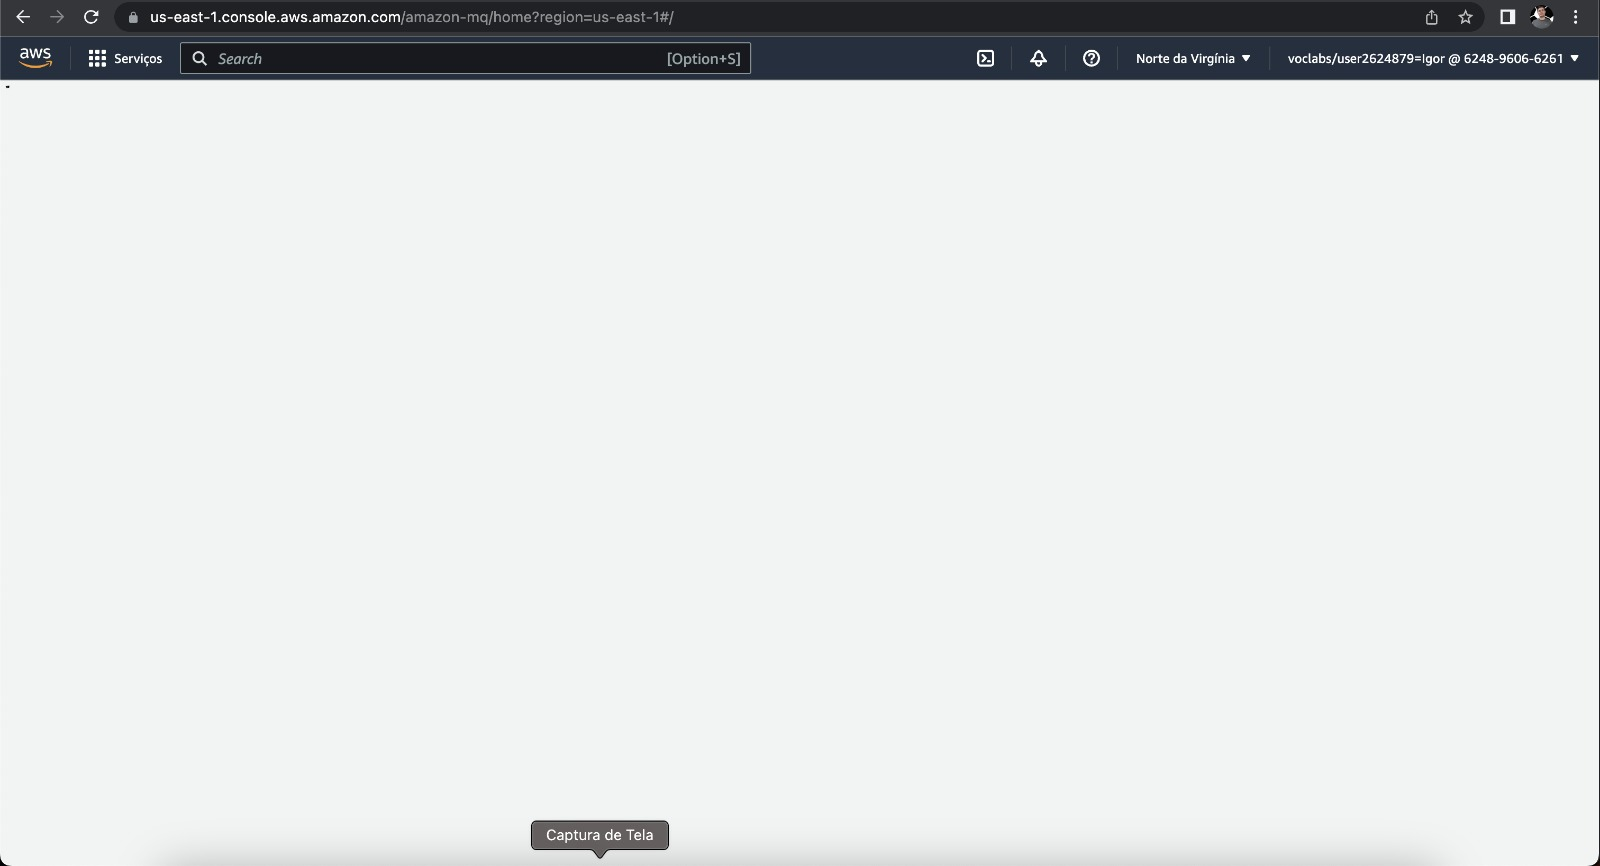
\includegraphics[scale = 0.25]{images/Erro Amazon MQ.jpeg}
    \caption{Tela ao tentar acessar o ambiente do AmazonMQ}
    \label{amazonmq}
\end{figure}

\section*{Modelagem da base de dados}

O sistema de monitoramento de rodovias consiste em uma evolução da versão entregue no último trabalho. A parte dos simuladores foi adaptada para respeitar os requisitos do trabalho, provocando indeterminismo na emissão dos eventos. Para tanto, as rodovias e os carros passaram a ser atualizados com threads. Além disso, como requisito do trabalho, a posição e demais informações do carro são emitidas logo após a atualização da posição do veículo. Já em relação ao processamento dos dados, descartamos todo o pipeline elaborado em C++ e implementamos um novo pipeline em Python, por meio da utilização do Spark (mais especificamente por meio da sua API para Python, o PySpark).

Visto que não desejamos perder nenhum evento emitido, optamos por armazenar os dados brutos em um banco NoSQL. O banco escolhido foi o MongoDB, pela facilidade de manuseio e por cumprir os requisitos. Uma vez que os dados estão no banco, o Spark lê os mesmos e transforma a informação, gerando as análises solicitadas. Em seguida, de modo a deixar modularizado o pipeline, carregamos as tabelas com as análises para um banco relacional, sendo cada tabela corresponde a uma análise. Por fim, com auxílio do \textit{streamlit}, geramos um Dashboard e exibimos tais análises.

\section*{Decisões de projeto}

A seguir listamos as principais decisões de projeto realizadas no trabalho.
\begin{itemize}
    \item Como opção para método de comunicação, escolhemos o Publish-Subscribe (Pub/Sub) por ser mais facilmente escalável do que o método RPC. A vantagem do Pub/Sub sobre o RPC é que este último requer uma operação síncrona e é geralmente mais lento. Além disso, descartamos o uso de um MPI pelo fato do Pub/Sub ter uma implementação mais fácil e mais adequada ao nosso projeto.

    \item Como escolhemos o modelo ELTL, precisávamos de um banco que armazenasse os dados brutos da etapa de extração para depois fazer o tratamento. Nesse sentido, um banco NoSQL é a opção ideal. Dentre os possíveis bancos, escolhemos trabalhar com o MongoDB. Tal escolha foi dada pela eficiência do MongoDB para lidar com registros de gravações intensivas\footnote{No nosso caso, os dados do mock, ao serem publicados, não devem sobrecarregar a memória.} e por ele ser horizontalmente escalável o que é muito conveniente a medida que o volume de rodovias aumenta.

    \item Para o armazenamento dos dados tratados, um banco relacional encaixa-se melhor. Novamente, dentre as opções, optamos pelo PostgreSQL. Tal escolha se deu pelo fato desse banco ser adapto trabalhar em projetos com grande volumes de dados e necessidade de escalabilidade. Outro ponto positivo para a escolha desse banco é o fácil acesso e manipulação do mesmo em Python via API.
    
    \item Para o Dashboard procuramos uma ferramenta simples, mas que fosse capaz de processar e realizar atualizações de forma eficiente. Diante disso escolhemos o \textit{streamlit}, uma biblioteca Python para construção e exibição de Dashboards capaz de acompanhar eficientemente o fluxo de atualizações dos dados. Além disso, o \textit{streamlit} é de fácil manuseio e atende perfeitamente os requisitos da disciplina.

    \item Por conta de diversas dificuldades em configurar o ambiente em nuvem, optamos por não subir o trabalho para o ambiente da AWS. Em contrapartida, priorizamos um melhor funcionamento do projeto de maneira geral, além de garantir que todos os outros requisitos sejam atingidos.
\end{itemize}

\section*{Resultado dos experimentos}

Por fim, realizamos as medições do tempo de processamento das análises realizadas. Além de disponibilizar no Dashboard o tempo de processamento de cada análise no momento de visualização, isto é, o tempo que a análise que está em tela levou para ser gerada, olhamos para o tempo médio histórico de cada análise, discriminando pelo número de rodovias instanciadas. Como a análise prioritária era para risco de colisão, focamos os gráficos, nesse relatório, para essa análise e para o tempo geral, entretanto os demais gráficos podem ser encontrados em anexo, além de estarem disponíveis no repositório que hospeda o trabalho.
\begin{figure}[H]
    \centering
    \includegraphics[scale = 0.6]{images/Colisão.png}
    \caption{Tempo médio de execução da análise de riscos de colisão de acordo com o número de rodovias.}
    \label{colision_time}
\end{figure}

Como podemos ver, o tempo médio de execução para a análise não está bem comportado para poucas rodovias, mas se mantém estável até termos 60 rodovias. Após isso podemos perceber uma nova instabilidade, mas com uma tendência de aumento. Tal tendência pode ser explicada pelo número de veículos presentes na simulação. Quanto maior o número de veículos, mais dados teremos para processar e, consequentemente, mais tempo é esperado para que os mesmos sejam processados. Conforme o número de rodovias aumenta, o número de carros também aumenta e, com isso, o tempo de processamento também é afetado, aumentando. Em relação ao tempo total (tempo levado para realização de todas as análises), o gráfico da Figura \ref{total_time} mostra que temos um comportamento similar ao observado para o tempo de cálculo do risco de colisão.

\begin{figure}[H]
    \centering
    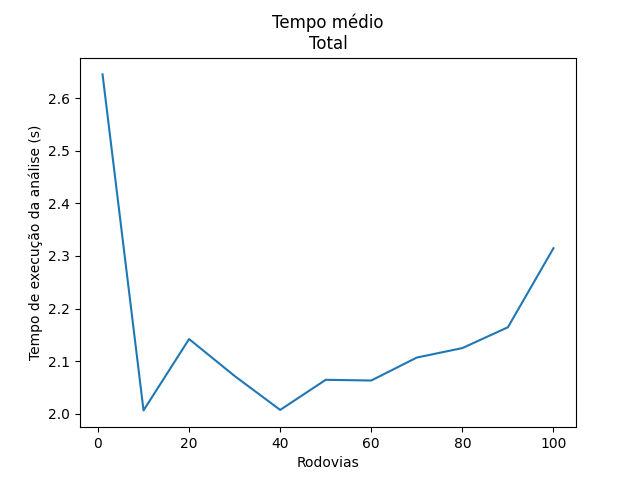
\includegraphics[scale = 0.6]{images/Total.png	}
    \caption{Tempo médio de execução do programa de maneira geral de acordo com o número de rodovias.}
    \label{total_time}
\end{figure}

Por fim, todo o histórico do trabalho e demais gráficos podem ser encontrados no repositório do trabalho \url{https://github.com/IgorMichels/Scalable_Computing}.

\end{document}